\section*{F\+E\+Mproject}

Trabaho Final da Disciplina de Introdução ao Método dos Elementos Finitos

\section*{Autores}


\begin{DoxyItemize}
\item Igor de Melo Nery de Oliveira
\item Lucas Gouveia Omena Lopes
\end{DoxyItemize}

\section*{Projeto Final}


\begin{DoxyItemize}
\item Implementação dos Elementos Finitos Q4 e T6 para resolução de um problema de uma estrutura submetida ao estado plano de tensões.
\end{DoxyItemize}

\section*{Problema Estudado}

Pilar engastado na base, e submetido a uma carga distribuída vertical no topo\+:

\subsection*{html /\+Figuras/problema.png}


\begin{DoxyImageNoCaption}
  \mbox{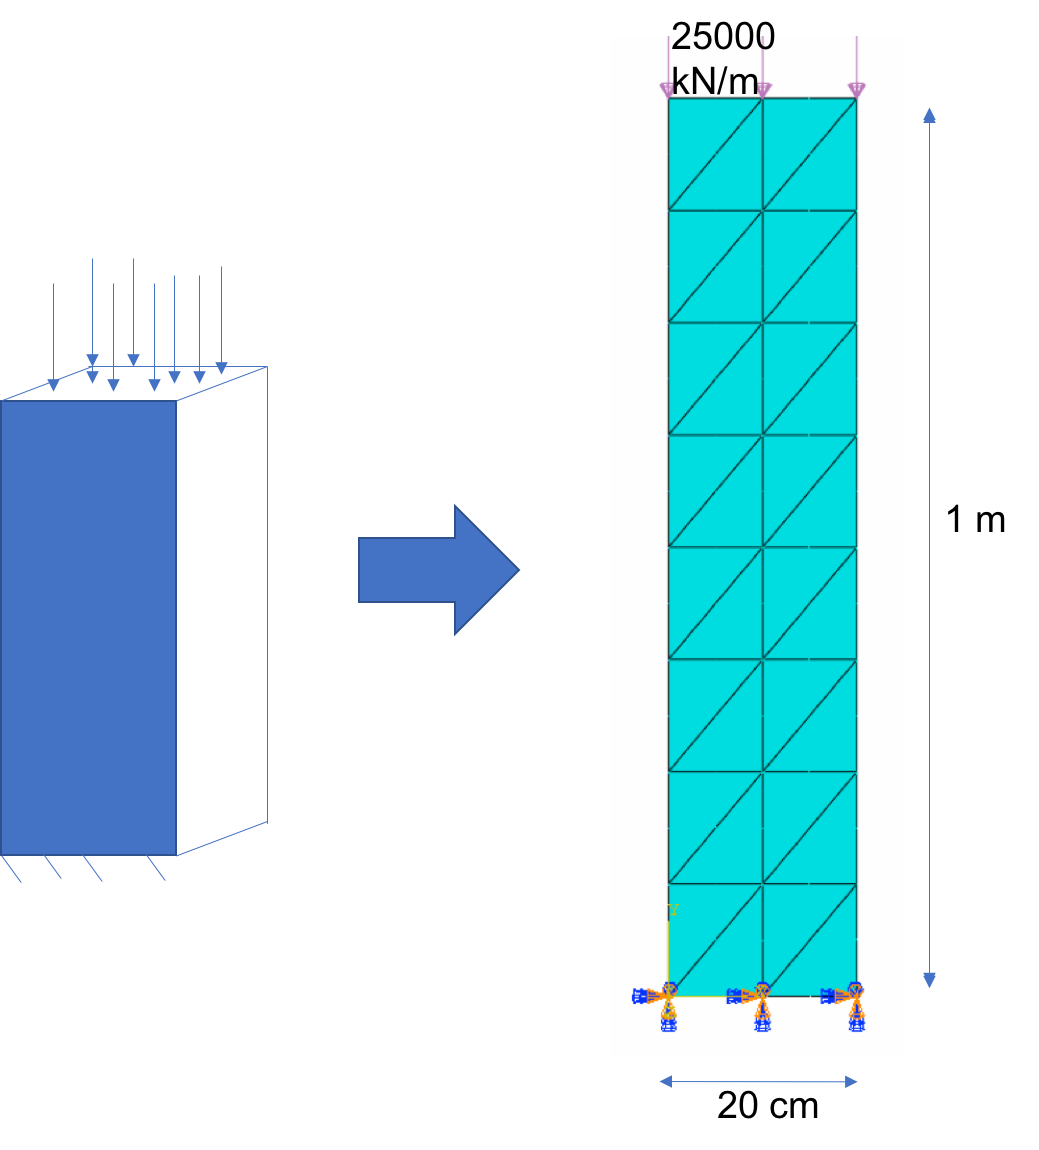
\includegraphics[width=\textwidth,height=\textheight/2,keepaspectratio=true]{problema.png}}
\end{DoxyImageNoCaption}
 

\section*{Elementos em Estudo}

\subparagraph*{Elemento Q4\+:}


\begin{DoxyItemize}
\item Elemento Quadilateral de 4 nós
\end{DoxyItemize}

\subsection*{html /\+Figuras/element\+Q4.png}


\begin{DoxyImageNoCaption}
  \mbox{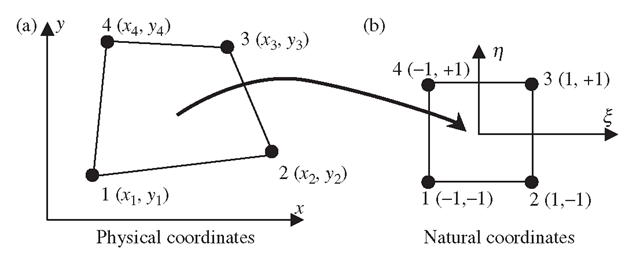
\includegraphics[width=\textwidth,height=\textheight/2,keepaspectratio=true]{elementQ4.png}}
\end{DoxyImageNoCaption}
 

\subparagraph*{Elemento T6\+:}


\begin{DoxyItemize}
\item Elemento Triangular de 6 nós
\end{DoxyItemize}

\subsection*{html /\+Figuras/\+T6.png}


\begin{DoxyImageNoCaption}
  \mbox{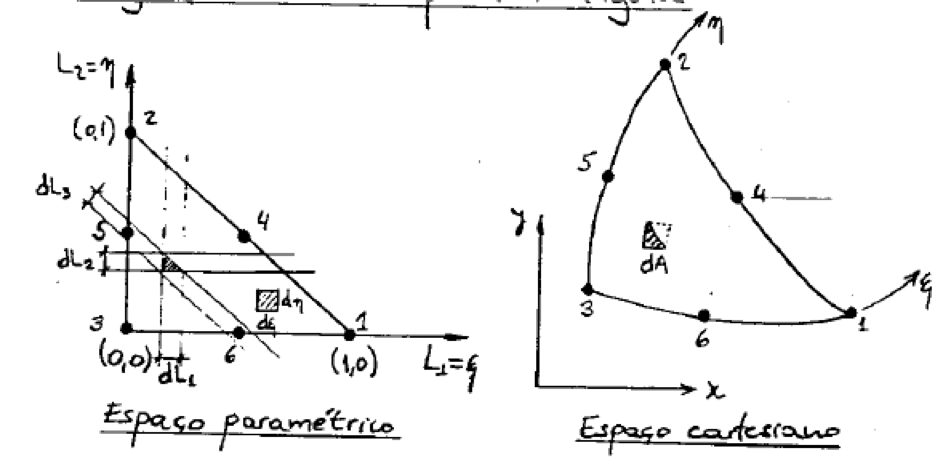
\includegraphics[width=\textwidth,height=\textheight/2,keepaspectratio=true]{T6.png}}
\end{DoxyImageNoCaption}
 

\section*{Objetivos}


\begin{DoxyItemize}
\item Implementação e uso dos elementos Q4 e T6 na resolução do problema proposto;
\item Avaliação dos resultadsos e comparação dos mesmos com os do software Abaqus.
\end{DoxyItemize}

\section*{Resultados}

\subsection*{Implementação Computacional dos Elementos T6 e Q4}


\begin{DoxyItemize}
\item As implementações dos elementos, juntamente com um código de análise de problemas usando o Método dos Elementos Finitos, foram feitas fazendo-\/se uso da linguagem de programação C++;
\item Os códigos e documentações seguem junto a esse P\+DF, podendo ser acessados de maneira iterativa através do arquivo H\+T\+ML, onde toda documentação e comentários se encontram.
\item A implementação apresentada faz uso do arquivo de entrada do software comercial Abaqus, afim de tirar proveito da ferramenta de geração de malhas do mesmo;
\item Os resultados obtidos através dessa implementação são verificados através do Abaqus, e serão apresentados posteriormente.
\end{DoxyItemize}

\subsection*{Abaqus}


\begin{DoxyItemize}
\item Foram testados exemplos, utilizando como material o aço (Modulo de Young 200 G\+Pa e coeficiente de Poisson 0.\+3), e estudados os efeitos do tipo de elemento e refinamento da malha nos resultados obtidos. Esses resultados, visulaizados através das ferramentas do software Abaqus. Os campos avaliados foram os deslocamentos (U),tensões (S), reações de apoio (RF) e deformações na estrutura (E).
\end{DoxyItemize}

\subsubsection*{Deslocamentos}

\subsubsection*{html /\+Figuras/45U.png}


\begin{DoxyImageNoCaption}
  \mbox{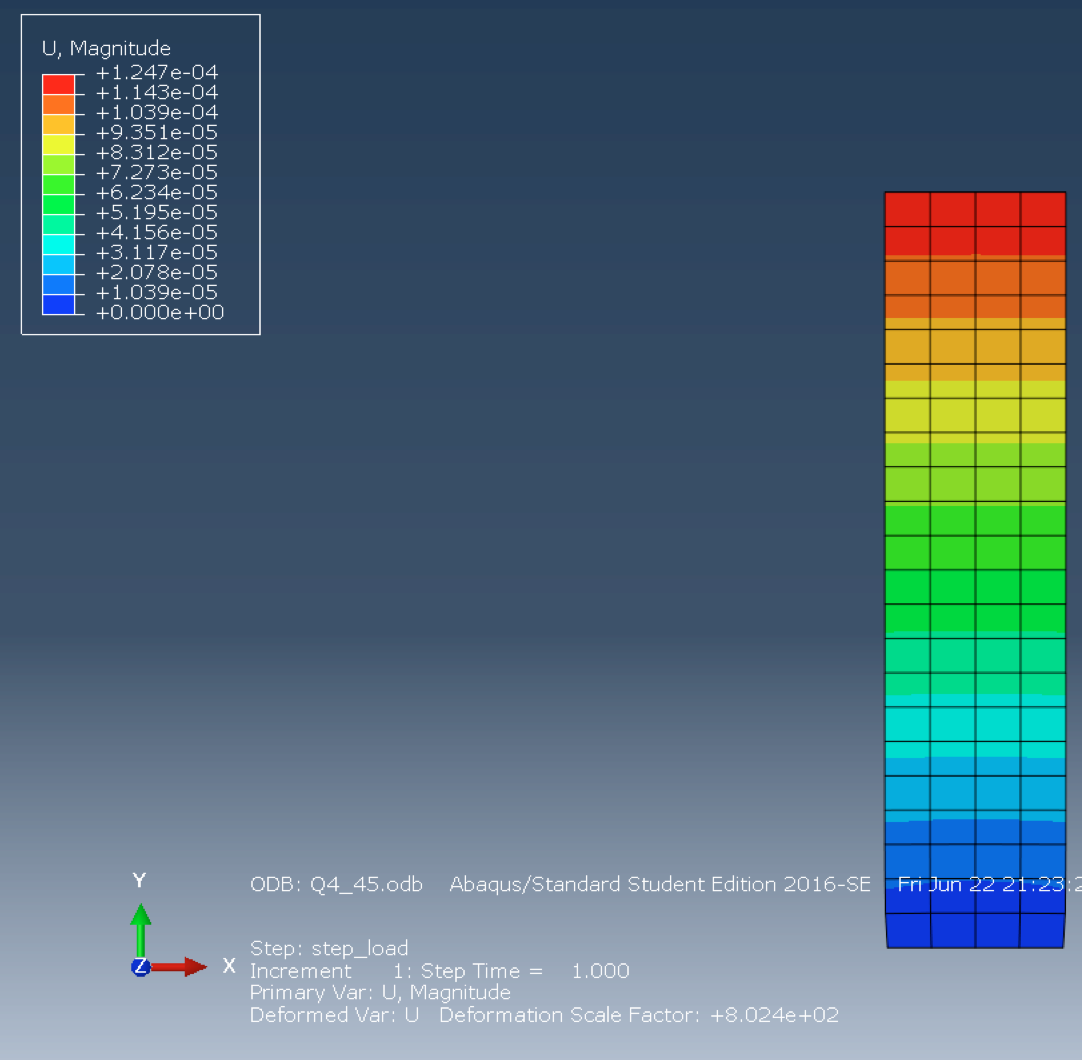
\includegraphics[width=\textwidth,height=\textheight/2,keepaspectratio=true]{45U.png}}
\end{DoxyImageNoCaption}
 

\subsubsection*{Tensões}

\subsubsection*{html /\+Figuras/45S.png}


\begin{DoxyImageNoCaption}
  \mbox{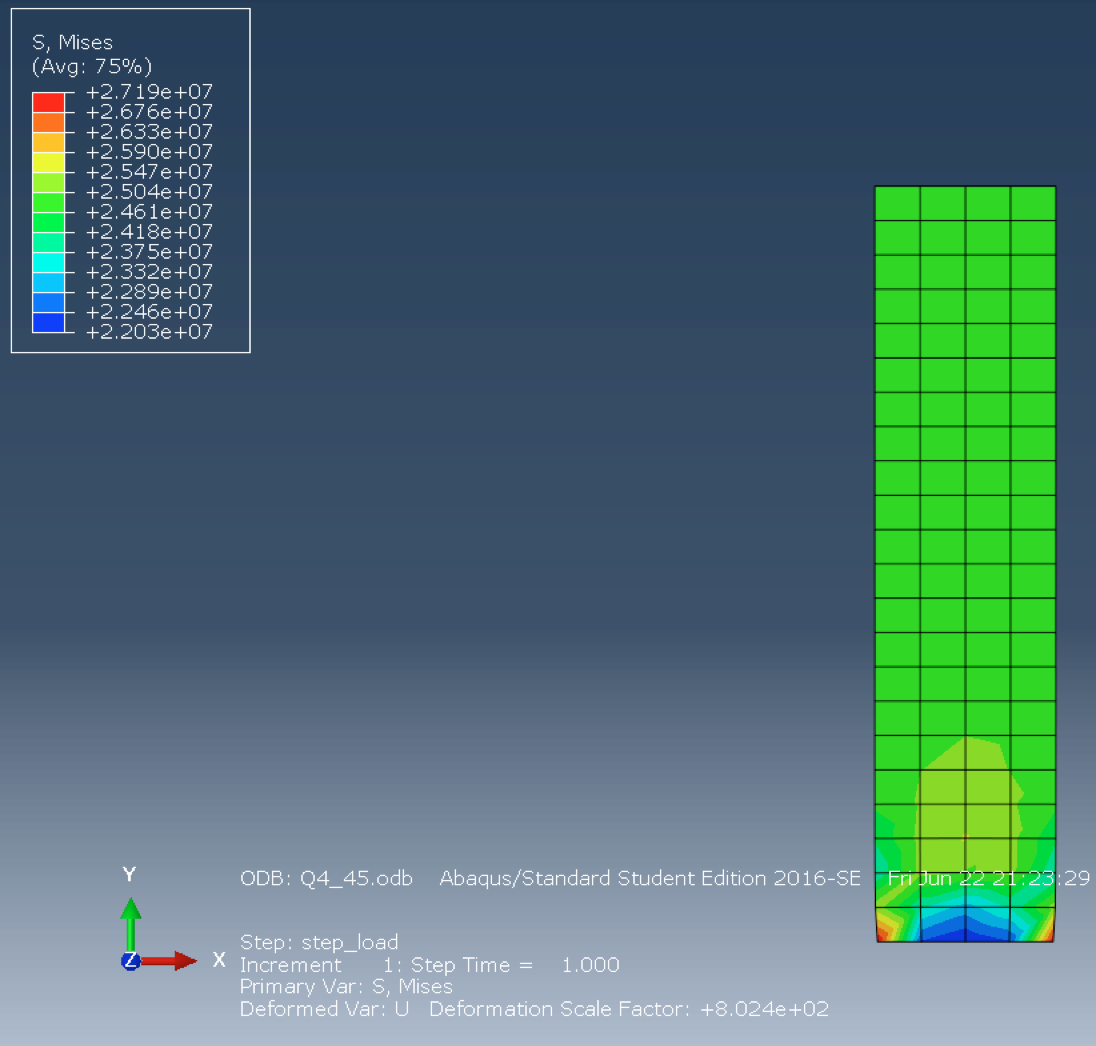
\includegraphics[width=\textwidth,height=\textheight/2,keepaspectratio=true]{45S.png}}
\end{DoxyImageNoCaption}
 

\subsubsection*{Reações}

\subsubsection*{html /\+Figuras/45\+RF.png}


\begin{DoxyImageNoCaption}
  \mbox{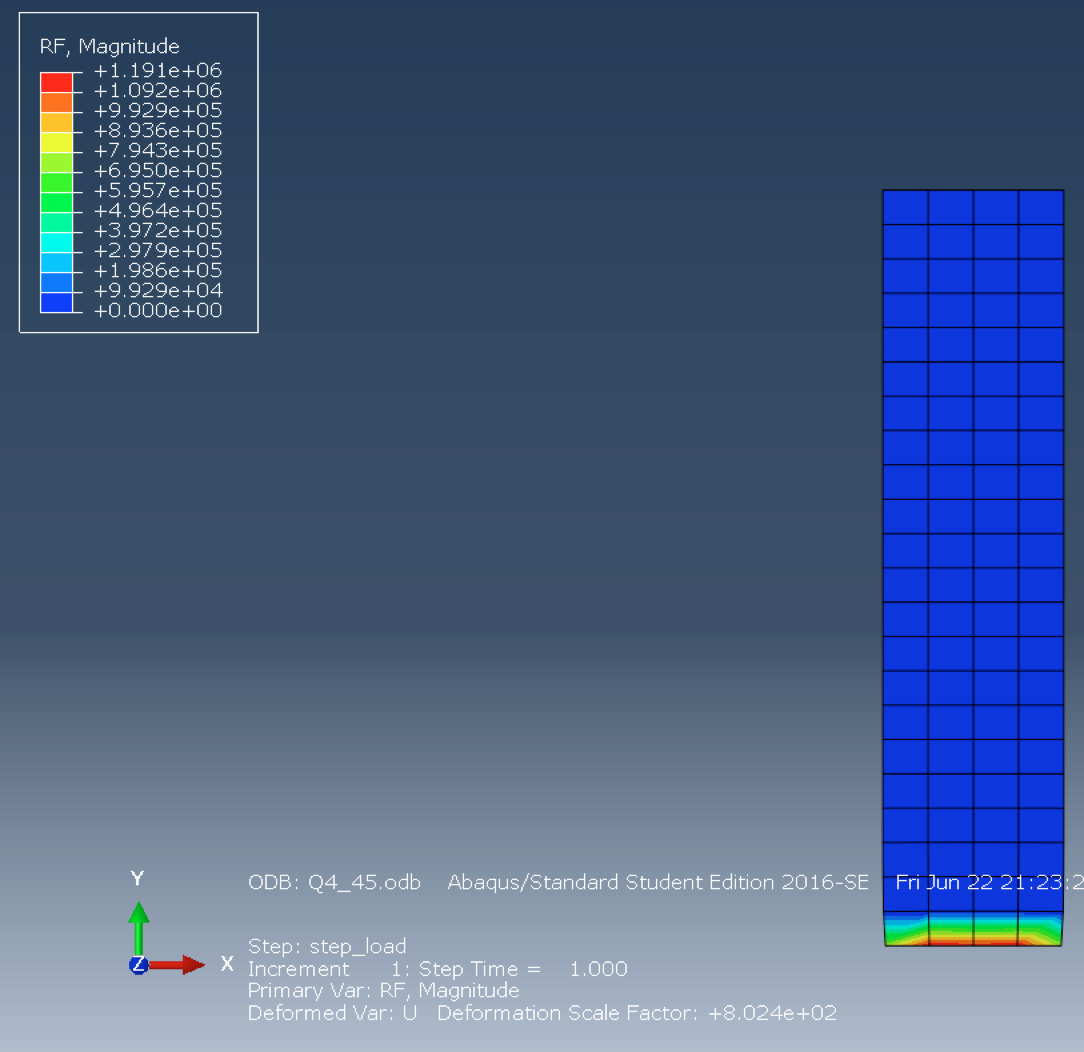
\includegraphics[width=\textwidth,height=\textheight/2,keepaspectratio=true]{45RF.png}}
\end{DoxyImageNoCaption}
 

\subsubsection*{Deformações}

\subsubsection*{html /\+Figuras/45E.png}


\begin{DoxyImageNoCaption}
  \mbox{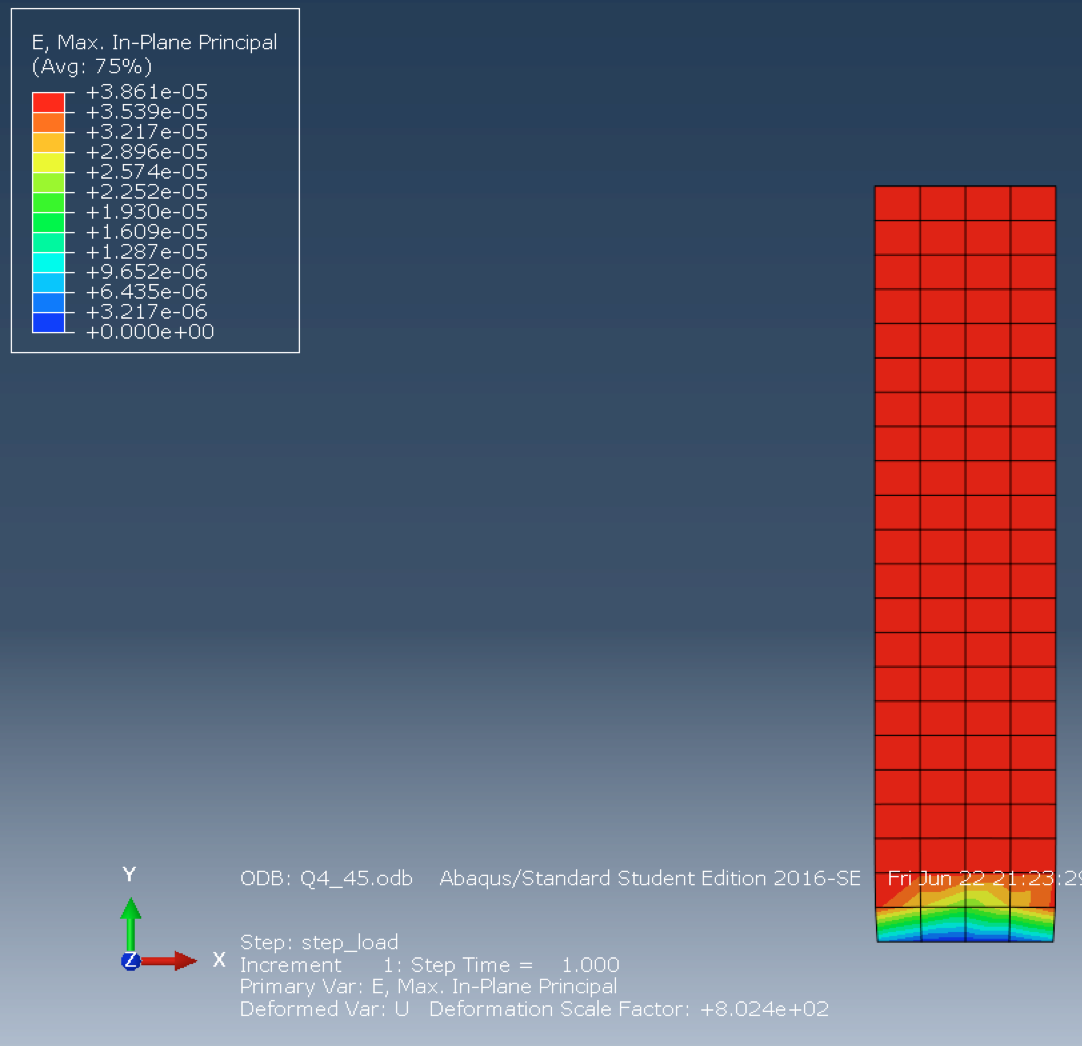
\includegraphics[width=\textwidth,height=\textheight/2,keepaspectratio=true]{45E.png}}
\end{DoxyImageNoCaption}
 

\subsection*{Influência do Número de Elementos}


\begin{DoxyItemize}
\item Para avaliarmos a interferência do refinamento da malha nos resultados obtidos, realizou-\/se um estudo das tensões e deformações medidas nos elementos. Esse estudo pode ser fisto nas figuras a seguir (simulações do Abqus para variadas divisões de elementos), e no gráfico, que mostra a influência do resultado de acordo com o número de elementos.
\end{DoxyItemize}

\subsubsection*{html /\+Figuras/tabela.png}


\begin{DoxyImageNoCaption}
  \mbox{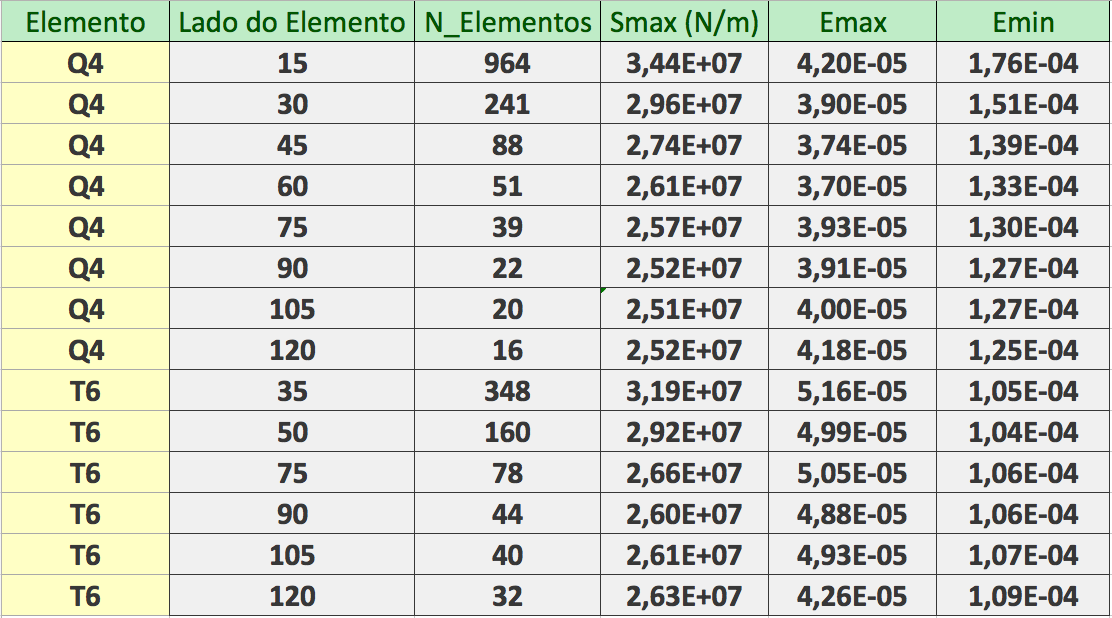
\includegraphics[width=\textwidth,height=\textheight/2,keepaspectratio=true]{tabela.png}}
\end{DoxyImageNoCaption}
 

\subsubsection*{Q4}

\subsubsection*{html /\+Figuras/stress.png}


\begin{DoxyImageNoCaption}
  \mbox{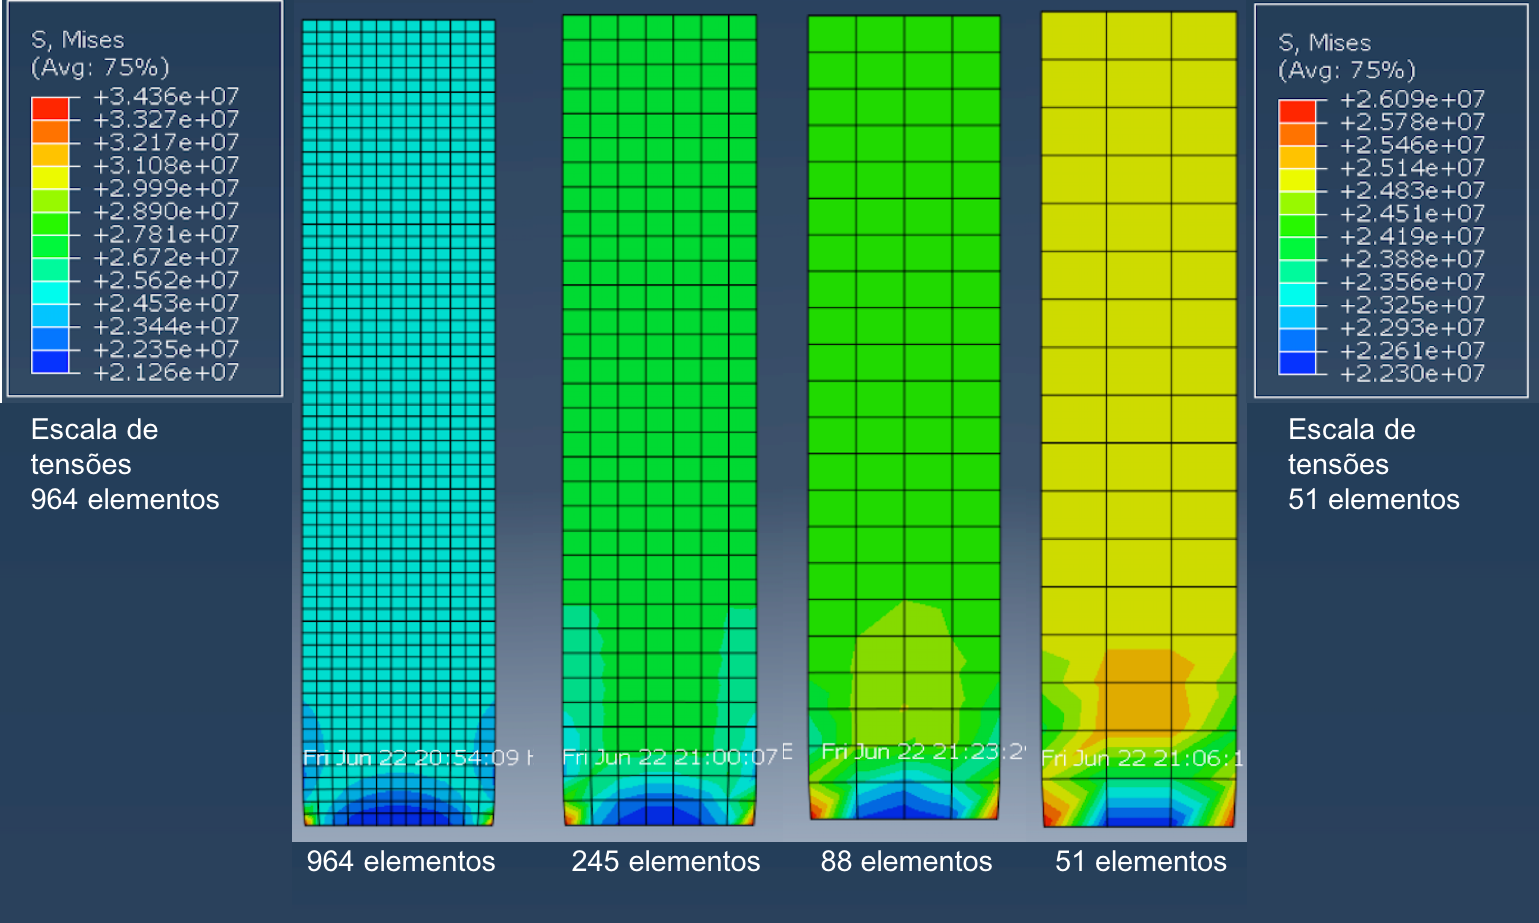
\includegraphics[width=\textwidth,height=\textheight/2,keepaspectratio=true]{stress.png}}
\end{DoxyImageNoCaption}
 

\subsubsection*{html /\+Figuras/strain.png}


\begin{DoxyImageNoCaption}
  \mbox{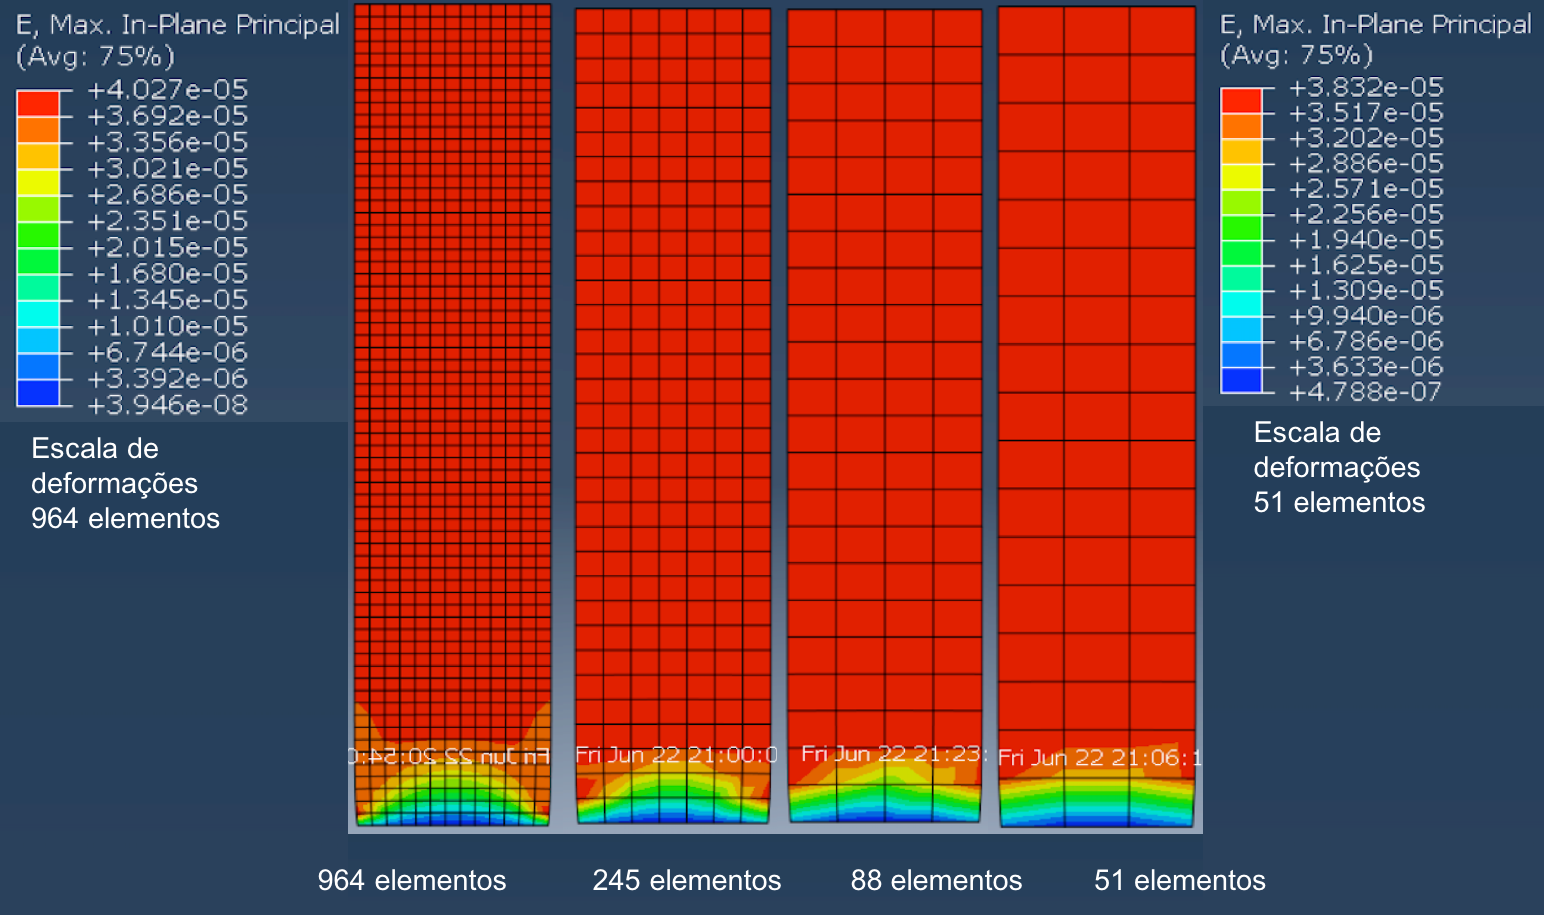
\includegraphics[width=\textwidth,height=\textheight/2,keepaspectratio=true]{strain.png}}
\end{DoxyImageNoCaption}
 

\subsubsection*{T6}

\subsubsection*{html /\+Figuras/stress\+\_\+t6.png}


\begin{DoxyImageNoCaption}
  \mbox{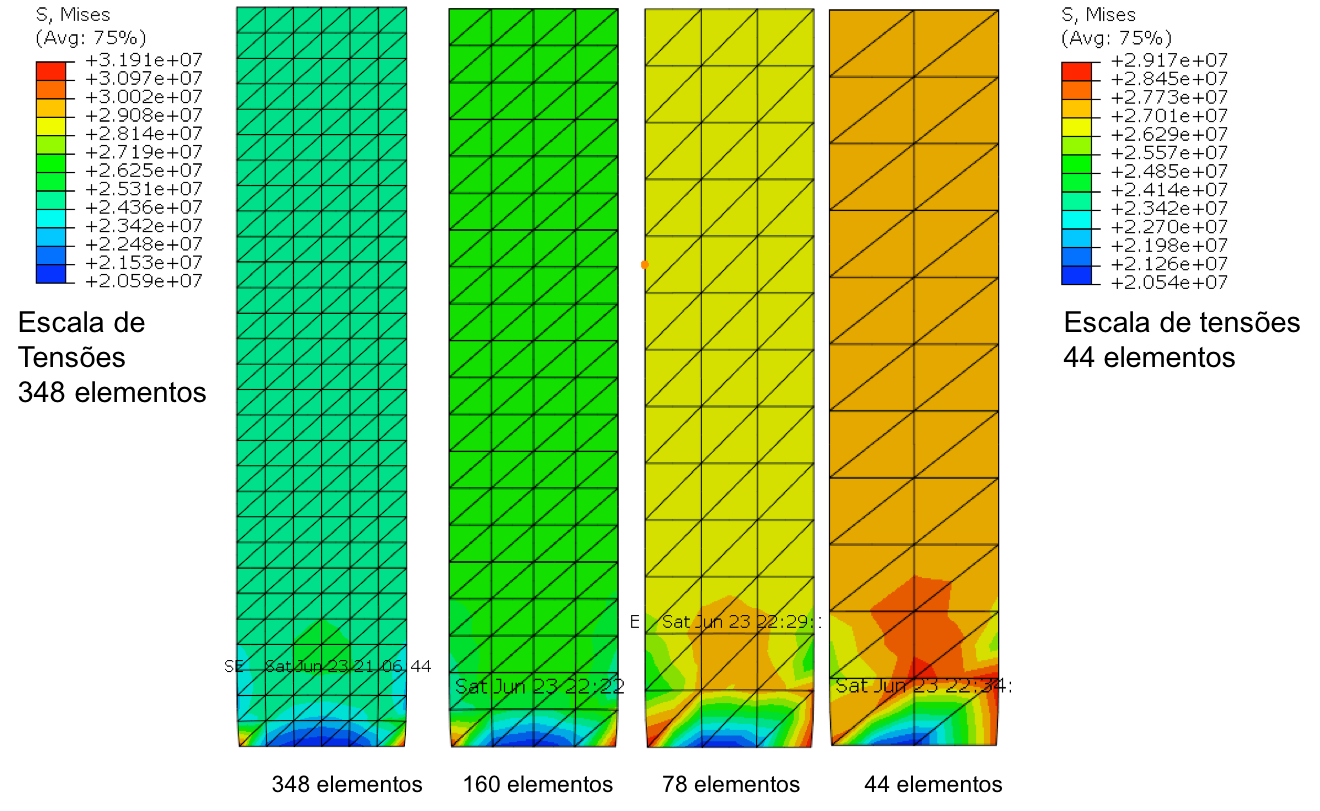
\includegraphics[width=\textwidth,height=\textheight/2,keepaspectratio=true]{stress_t6.png}}
\end{DoxyImageNoCaption}
 

\subsubsection*{html /\+Figuras/strain\+\_\+t6.png}


\begin{DoxyImageNoCaption}
  \mbox{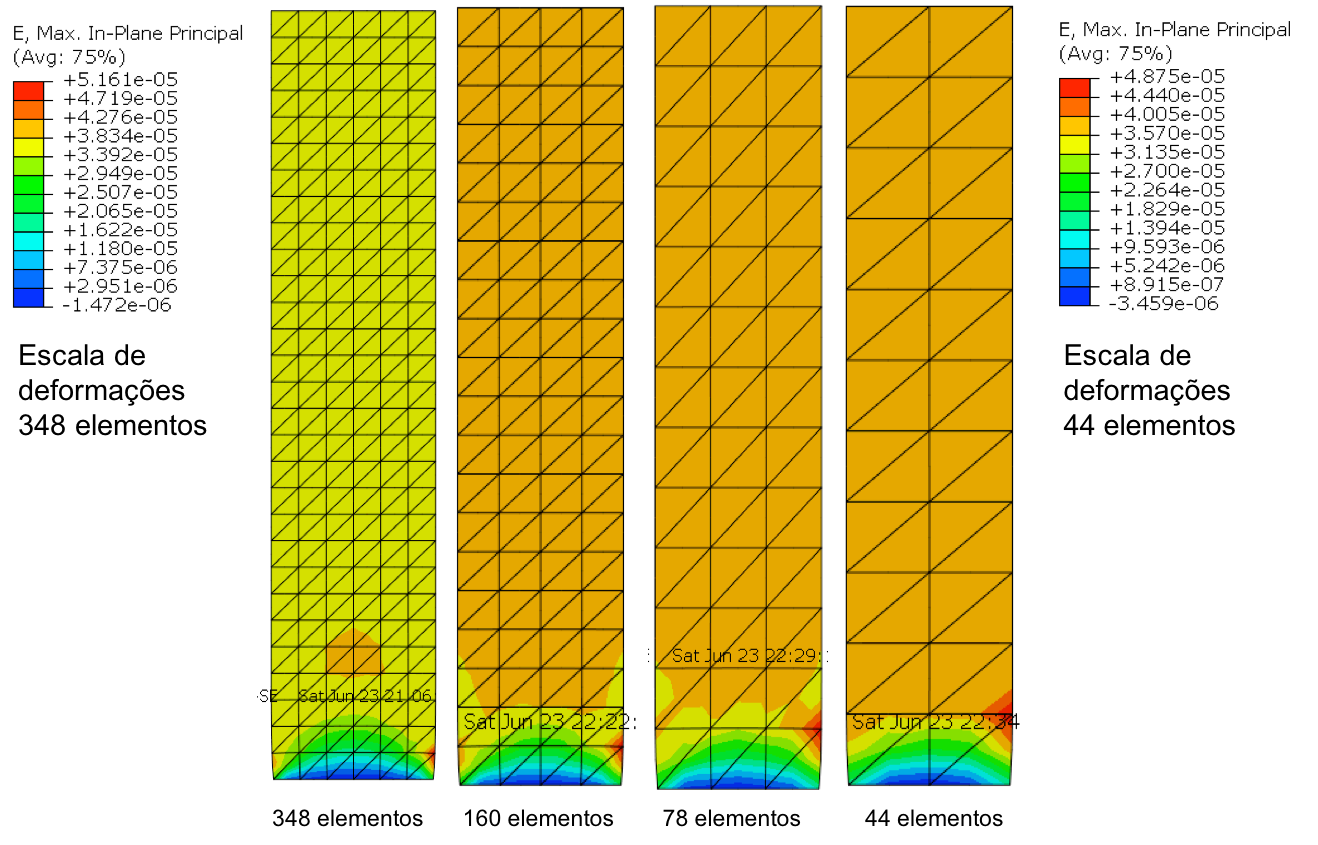
\includegraphics[width=\textwidth,height=\textheight/2,keepaspectratio=true]{strain_t6.png}}
\end{DoxyImageNoCaption}
 

\subsection*{Gráfico Número de Elementos x Tensões Máximas}

\subsubsection*{Q4}

\subsubsection*{html /\+Figuras/q4\+\_\+elementxstress.png}


\begin{DoxyImageNoCaption}
  \mbox{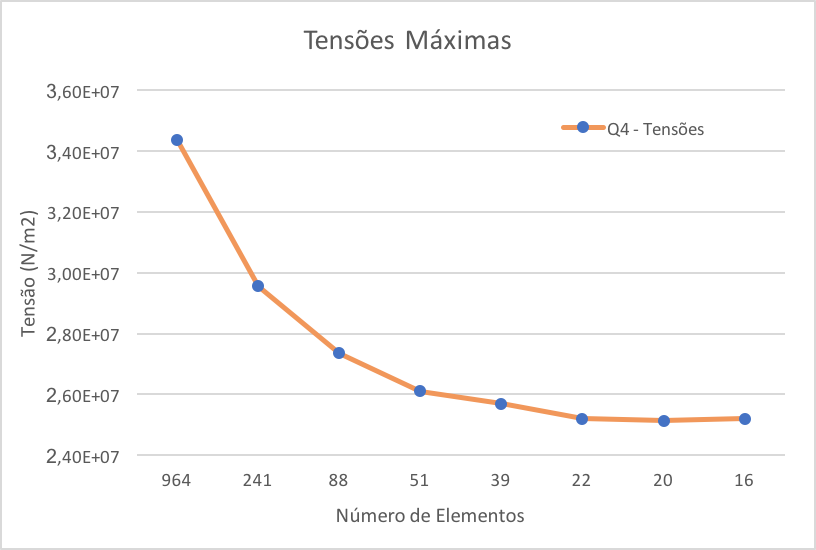
\includegraphics[width=\textwidth,height=\textheight/2,keepaspectratio=true]{q4_elementxstress.png}}
\end{DoxyImageNoCaption}
 

\subsubsection*{T6}

\subsubsection*{html /\+Figuras/t6\+\_\+elementxstress.png}


\begin{DoxyImageNoCaption}
  \mbox{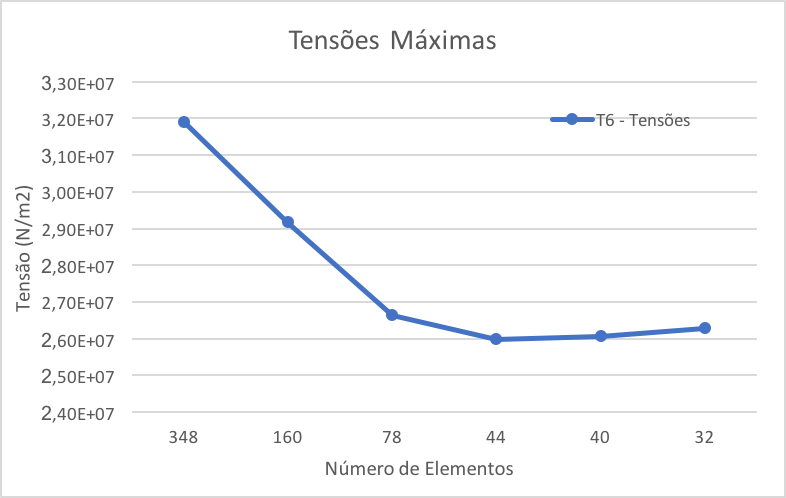
\includegraphics[width=\textwidth,height=\textheight/2,keepaspectratio=true]{t6_elementxstress.png}}
\end{DoxyImageNoCaption}
 

\subsection*{Gráfico Número de Elementos x Deformações Máximas}

\subsubsection*{Q4}

\subsubsection*{html /\+Figuras/q4\+\_\+elementxstrain.png}


\begin{DoxyImageNoCaption}
  \mbox{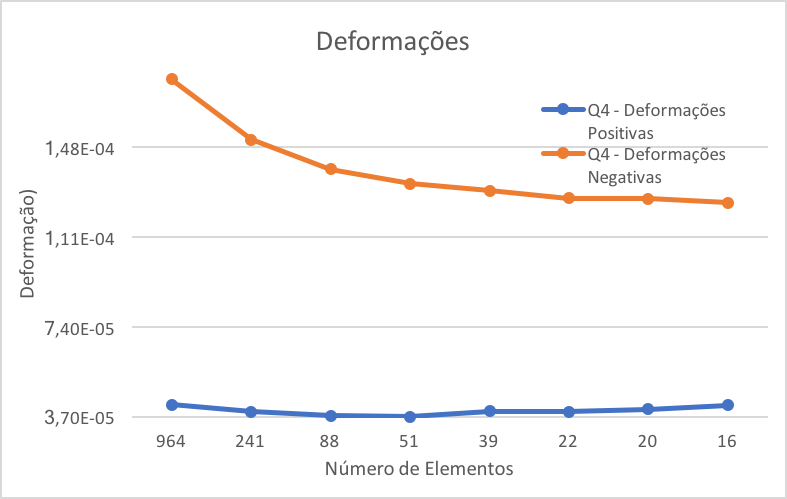
\includegraphics[width=\textwidth,height=\textheight/2,keepaspectratio=true]{q4_elementxstrain.png}}
\end{DoxyImageNoCaption}
 

\subsubsection*{T6}

\subsubsection*{html /\+Figuras/t6\+\_\+elementxstrain.png}


\begin{DoxyImageNoCaption}
  \mbox{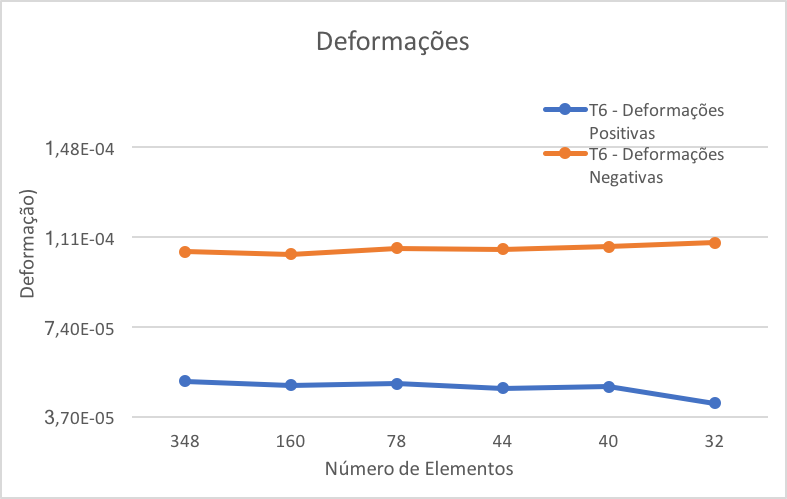
\includegraphics[width=\textwidth,height=\textheight/2,keepaspectratio=true]{t6_elementxstrain.png}}
\end{DoxyImageNoCaption}
 

\section*{Análise dos resultados}


\begin{DoxyItemize}
\item A partir dos resultados, avaliou-\/se a influência do refinamento da malha nos resultados das análises de elementos finitos. Malhas mais refinadas, além de fornecerem resultados com maior grau de suavidade e continuidade, apresentão um comportamento menos rígido em relação as malhas menos refinadas. Apesar de ser uma diferença não tão pronunciada, foi observado que elementos mais refinados tem tanto deformações quanto tensões mais acentuadas.
\item Foi constatado também que, para os elementos do tipo T6, a qualidade da resposta é inferior ao Q4, apesar das funções de interpolação quadrádicas utilizadas.
\end{DoxyItemize}

\subsection*{Referencias até o momento}

\href{http://eigen.tuxfamily.org/index.php?title=IDEs#Visual_Studio}{\tt Eigen Website -\/ Instalation} 